\documentclass[conference]{IEEEtran}
\usepackage{amsmath,amssymb,booktabs,graphicx,url}
\usepackage{pgfplots}
\usepgfplotslibrary{groupplots}
\pgfplotsset{compat=1.18}
\definecolor{modelblue}{HTML}{2468A6}
\definecolor{modelorange}{HTML}{C66A28}
\definecolor{modelgreen}{HTML}{16826E}
\definecolor{modelpurple}{HTML}{7957A8}
\definecolor{modelrose}{HTML}{B23C74}
\graphicspath{{./}{paper1_action/}}
\title{When Does a Spiking Decision Core Help? A Controlled Study of Spoken Action Selection}
\author{\begin{tabular}{cc}
\parbox{0.46\textwidth}{\centering\textbf{Abiel M. Berhanu}\\
\textit{Electrical and Computer Engineering}\\University of Oklahoma\\
Norman, OK, United States\\abiel.m.berhanu-1@ou.edu} &
\parbox{0.46\textwidth}{\centering\textbf{Steven Di Jorio}\\
\textit{Stephenson School of Biomedical Engineering}\\University of Oklahoma\\
Norman, OK, United States\\steven.dijorio@ou.edu}\\[1.5em]
\parbox{0.46\textwidth}{\centering\textbf{Sarah Sharif}\\
\textit{Electrical and Computer Engineering}\\University of Oklahoma\\
Norman, OK, United States\\sarah.sharif@ou.edu} &
\parbox{0.46\textwidth}{\centering\textbf{Yaser Banad}\\
\textit{Electrical and Computer Engineering}\\University of Oklahoma\\
Norman, OK, United States\\bana@ou.edu}
\end{tabular}}
\begin{document}
\maketitle

\begin{abstract}
Voice interfaces must choose an application action from uncertain speech and sometimes defer. We compare a spiking leaky integrate-and-fire decision core with plain and leak-matched tanh recurrent networks and a gated recurrent unit (GRU), using frozen acoustic states and recognized words. Five-seed SLURP results show that matching leak removes the apparent spiking advantage on acoustic input; the GRU is strongest there. A prospectively fixed French Speech-MASSIVE replication preserves the acoustic ranking. On recognized French words, spiking has a small mean lead over leaky tanh, but a seed-and-utterance interval includes zero; a GRU and a simple word-and-phrase classifier score higher. The classifier also has the best selective risk and simulated action cost on SLURP ASR words. Deferral reduces wrong executions at substantial coverage cost. A secondary phone-command stress test reveals low correct-execution coverage. These offline results characterize decision-model tradeoffs without establishing an energy or accessibility benefit.
\end{abstract}

\begin{IEEEkeywords}
neuromorphic decision making, spiking neural networks, action selection, spoken language understanding, selective classification
\end{IEEEkeywords}

\section{Introduction}
A voice interface ultimately has to choose an action, not merely produce words. The relevant output may be one of a bounded set of operations such as setting an alarm, changing audio volume, or querying a calendar. A practical decision layer should also expose uncertainty so the application can defer rather than execute a low-confidence action. This work asks whether a brain-inspired spiking recurrent network can serve as that decision layer, and what it gains or loses relative to ordinary recurrent models when input comes from audio or recognized text.

The interface studied here is $x\mapsto(p(a_1\mid x),\ldots,p(a_K\mid x))$, followed by an action-or-defer rule. It is intentionally independent of any proprietary decision system. The acoustic branch uses a frozen pretrained encoder; the text branch receives actual ASR output from the same audio. Correct corpus transcripts provide an oracle diagnostic. This design separates the effect of the decision core from errors and computation in upstream speech processing.

The paper contributes (i) a five-seed comparison of spiking, plain tanh, leak-matched tanh, and gated recurrent decision cores on paired SLURP audio and text inputs; (ii) an independently recorded French speech benchmark and nonrecurrent text and acoustic controls; and (iii) calibrated-probability, selective-action, and hypothetical action-cost analyses. A secondary speaker-disjoint phone-command corpus tests the action interface in an accessibility setting; it is not a medical outcome study. The principal contribution is the measured decision-model tradeoff, including a negative result for a spiking-specific acoustic advantage. No edge-device or physical-energy result is claimed.

\section{Related Work}
SLURP supplies paired speech, transcripts, and scenario/action annotations for spoken-language understanding~\cite{slurp}. Prior work already compares acoustic, text, and richer ASR representations for SLURP intent detection~\cite{representations}; direct audio-to-intent learning itself is not new. Our comparison holds the decision input and action catalog fixed while changing the recurrent decision core, then evaluates confidence and deferral. Whisper supplies the frozen speech representation and the ASR hypotheses~\cite{whisper}; the upstream model is much larger than any decision core.

Surrogate gradients are an established way to train spiking networks through discrete firing events~\cite{neftci}. The Heidelberg spiking audio datasets support systematic temporal benchmarking~\cite{cramer}; adaptive spiking recurrent networks have improved speech and gesture classification~\cite{yin}; and Bittar and Garner compare surrogate-gradient spiking models with conventional speech-command baselines~\cite{bittar}. Blouw \emph{et al.} measure keyword-spotting efficiency on Loihi~\cite{blouw}, a hardware question outside this experiment. Earlier spiking action-decision studies include biologically inspired reinforcement-learning controllers~\cite{basal}. Work by Banad and colleagues uses spiking networks for online control with local plasticity~\cite{banad_cloud} and for integrated state estimation and control with recurrent LIF neurons~\cite{banad_control}. Those systems address dynamical control; here we study supervised choice among discrete application actions with a defer option. Temperature scaling is a standard post-hoc calibration method~\cite{guo}, and confidence-based rejection has a substantial selective-classification literature~\cite{selective}. Our development-set threshold reports an empirical operating point, not a probabilistic guarantee. EasyCall was collected for voice-operated smartphone communication and includes commands, close-sounding noncommands, speakers with dysarthria, and control speakers~\cite{easycall}.

\section{Bounded Action-Decision Method}
\subsection{Action Interface}
Let $\mathcal A=\{a_1,\ldots,a_K\}$ be the application action catalog and $x_{1:T}$ an input sequence. The decision core produces logits $z=f_\theta(x_{1:T})$. A scalar temperature $\mathcal T>0$ fitted on development data yields $p_k=\mathrm{softmax}(z/\mathcal T)_k$. The nominal decision rule is
\begin{equation}
\hat a(x)=\begin{cases}
\arg\max_{a_k\in\mathcal A}p_k,&\max_k p_k\geq\tau,\\
\mathrm{defer},&\max_k p_k<\tau.
\end{cases}
\end{equation}
Development predictions are sorted by descending maximum probability. We choose the largest accepted prefix whose cumulative empirical error does not exceed 10\% and set $\tau$ to its lowest confidence. Ties can slightly change coverage. This is a development-set operating point, not a test guarantee. ``Defer'' is a policy output, not a SLURP ground-truth class. In EasyCall, \emph{no\_action} is additionally a genuine labeled class; the execution threshold is chosen to limit development-set false execution on its noncommands to 1\%.

\subsection{Decision Cores}
The 64-unit spiking core has analog input projection, recurrent leaky integrate-and-fire (LIF) neurons, and an analog action readout. With projected input $u_t$, previous post-reset voltage $v_{t-1}$, and hidden spike vector $s_{t-1}$, its update is
\begin{equation}
\begin{aligned}
\tilde v_t&=0.9v_{t-1}+u_t+W_rs_{t-1},\\
s_t&=H(\tilde v_t-\vartheta),\qquad \vartheta=1,\\
v_t&=\tilde v_t-s_t.
\end{aligned}
\end{equation}
The forward $H$ fires at threshold $\vartheta=1$; backpropagation uses the surrogate derivative $(1+5|\tilde v_t-1|)^{-2}$. The readout consumes the concatenation of mean hidden activity and final hidden state. The plain 64-unit tanh network uses $h_t=\tanh(u_t+W_rh_{t-1})$. A leak-matched control instead maintains $m_t=0.9m_{t-1}+u_t+W_rh_{t-1}$ and emits $h_t=\tanh(m_t)$. It matches the spiking core's recurrent initialization gain of 0.25, while the plain tanh core uses 0.8. All three use the same readout and parameter count. A 47-unit GRU stays within 3\% of that count. A mean-plus-max-pooled linear probe provides a nonrecurrent acoustic control. The acoustic spiking and tanh cores each have 36,476 trainable parameters; the GRU has 37,331 and the linear probe 46,140. The text spiking and tanh cores each have 254,972 parameters, mostly token embeddings; the GRU has 261,539.

The SNN is not fully event-driven: its input projection and readout are analog, and its software implementation executes dense matrix operations at every sequence step. Mean hidden firing rate is reported as activity only. The SNN objective adds $0.002$ times mean firing rate to cross-entropy; nonspiking controls use cross-entropy alone. The leaky tanh core matches leak and initial gain, but the firing threshold, reset, and activity term still differ. No single ablation isolates every neuron mechanism.

\subsection{Input Representations}
For direct audio, one real SLURP recording is chosen deterministically per utterance. The English Whisper tiny encoder is frozen. Feature extraction and encoding use the recording's variable duration rather than a 30-second padded window; a 2.72-second clip produces 137 encoder states in our implementation. Only the resulting valid states are uniformly pooled or interpolated to 32 vectors of width 384, then normalized using training-split statistics. For recognized text, the same recording is transcribed by Whisper tiny.en at int8 precision with beam size one. The primary text cores are trained on official reference transcripts and evaluated on ASR hypotheses after development-set recalibration. A separate matched variant trains on ASR hypotheses from training recordings. Text is lowercased and tokenized to at most 40 tokens with a training-derived 5,000-token vocabulary and 48-dimensional embeddings. A word/bigram TF--IDF logistic classifier with at most 5,000 features and $C=1$ is a nonrecurrent text control. The paper reports ASR word error rate. The audio and text paths share the recordings and action labels, but their upstream computational costs differ. Whisper tiny has approximately 39 million parameters as a full ASR model~\cite{whisper}; it is not included in the decision-core counts.

\section{Experimental Protocol}
\subsection{Primary Benchmark and Training}
SLURP's official train/development/test partitions contain 11,514/2,033/2,974 utterances. We concatenate each annotated scenario and action into one of 60 distinct choices, matching the dataset authors' \emph{Scen\_Act} label definition~\cite{slurp}. All test choices occur in training. Only real audio is used, with one recording per utterance; no utterance ID or selected recording crosses splits. Six test sentences exactly match a training sentence after lowercasing and trimming. The official split is utterance-based, and we make no speaker-disjoint claim. The largest training action is 810 examples; the smallest is four. Always choosing the majority action yields 7.03\% test accuracy.

The models use AdamW, batch size 128, weight decay 0.001, norm-one gradient clipping, and seeds 11, 13, 17, 19, and 23. The learning rate is 0.0015 for acoustic states and 0.002 for text. Acoustic training runs at most 24 epochs and text at most 18, retaining the lowest development negative log-likelihood with early stopping. The same preprocessing, split, action catalog, and training budget are used within each recurrent comparison. Temperatures and defer thresholds are fitted only on development data. Reported measures are test action accuracy, macro F1, 15-bin expected calibration error (ECE), negative log-likelihood, selective coverage/error, and area under the risk--coverage curve (AURC). A paired hierarchical bootstrap resamples both seeds and utterances 5,000 times for accuracy differences. The five fixed seeds still do not encompass architecture or dataset uncertainty.

\subsection{Prospective French Speech Benchmark}
Speech-MASSIVE provides newly recorded multilingual speech for 60 intents based on the MASSIVE ontology~\cite{speechmassive}. We use French recordings with a frozen multilingual Whisper tiny encoder, the same valid-state pooling, the four recurrent cores, and the fixed training recipe above. Only recordings marked validated are included, excluding 34 files. We stratify the official training split into 10,333 fit and 1,149 internal-development recordings using seed 20261101. The official test files required authentication during this study, so we reserved the 2,031 validated official-validation recordings for final evaluation and fixed this substitution before inspecting its outcomes. For the recognized-word extension, the same 60-intent catalog and five seeds are used. Text models train on intended prompts, while multilingual Whisper tiny generates French hypotheses for development recalibration and final evaluation. A word/bigram TF--IDF logistic fit is a nonrecurrent control. Word error rate here is measured against intended prompts, not independently verified transcriptions. The French audio and speakers are independent of SLURP's, while the translated intent ontology descends from SLURP; this is a new-language recording and language replication, not a fully independent semantic task.

\subsection{Secondary Voice-Access Benchmark}
EasyCall contains 21,386 Italian recordings from 31 dysarthric and 24 control speakers~\cite{easycall}. The authors' listed executable phrases are mapped to 35 phone actions, while 30 close-sounding noncommand prompts map to \emph{no\_action}; the ontology is specified in our experiment code. Speaker-disjoint train/development/test partitions contain 33/11/11 speakers and 13,115/4,118/4,153 recordings, respectively. Audio is resampled to 16 kHz and represented as 48 frames of 40 log-mel features. A common two-layer convolutional acoustic front end feeds a spiking or tanh decision core, each with 38,372 trainable parameters. Both models use class-weighted cross-entropy and seeds 11, 13, and 17. We report action accuracy and macro F1 by speaker group, plus false executions on noncommands and correct executions on commands. The files identify intended prompts, not independently verified words spoken. There is no live device interaction or user benefit measure.



\begin{table*}[t]
\caption{SLURP action selection on 2,974 official test utterances. ASR-word models in this table were trained on reference transcripts. Accuracy and macro F1 are mean $\pm$ sample standard deviation across five seeds. Coverage and accepted-error columns use thresholds selected for $\leq$10\% empirical development accepted error; test error can exceed 10\%. Linear probe is one deterministic fit. Decision parameter counts exclude the frozen Whisper upstream model.}
\label{tab:slurp}
\centering\scriptsize
\begin{tabular}{llrrrrr}
\toprule
Input state & Decision core & Parameters & Accuracy (\%) & Macro F1 (\%) & Coverage (\%) & Accepted error (\%)\\
\midrule
Frozen audio states & tanh RNN & 36,476 & $42.95\pm0.67$ & $30.91\pm1.43$ & 11.67 & 10.97\\
Frozen audio states & leaky tanh RNN & 36,476 & $50.64\pm0.48$ & $41.35\pm1.07$ & 21.65 & 10.30\\
Frozen audio states & spiking LIF RNN & 36,476 & $50.48\pm0.33$ & $41.04\pm0.71$ & 23.30 & 11.42\\
Frozen audio states & GRU & 37,331 & $55.12\pm0.63$ & $44.61\pm1.08$ & 31.55 & 11.63\\
Frozen audio states & linear probe & 46,140 & 51.68 & 45.52 & 26.26 & 10.88\\
\midrule
ASR words & tanh RNN & 254,972 & $54.66\pm0.69$ & $48.91\pm1.40$ & 37.09 & 11.04\\
ASR words & leaky tanh RNN & 254,972 & $56.19\pm0.53$ & $51.51\pm0.81$ & 39.74 & 10.38\\
ASR words & spiking LIF RNN & 254,972 & $57.46\pm0.40$ & $52.78\pm0.83$ & 41.47 & 11.01\\
ASR words & GRU & 261,539 & $57.30\pm0.84$ & $52.77\pm1.24$ & 41.98 & 11.05\\
\midrule
Oracle transcript & tanh RNN & 254,972 & $75.06\pm0.28$ & $68.37\pm1.11$ & 72.19 & 10.66\\
Oracle transcript & leaky tanh RNN & 254,972 & $77.05\pm0.66$ & $71.80\pm0.76$ & 77.05 & 10.77\\
Oracle transcript & spiking LIF RNN & 254,972 & $77.53\pm0.37$ & $72.62\pm0.80$ & 78.00 & 11.17\\
Oracle transcript & GRU & 261,539 & $77.59\pm0.52$ & $71.93\pm0.78$ & 78.59 & 11.16\\
\bottomrule
\end{tabular}
\end{table*}

\begin{figure*}[!t]
\centering
\IfFileExists{accuracy_comparison.png}{%
\includegraphics[width=0.98\textwidth]{accuracy_comparison.png}%
}{\IfFileExists{paper1_action/accuracy_comparison.png}{%
\includegraphics[width=0.98\textwidth]{paper1_action/accuracy_comparison.png}%
}{%
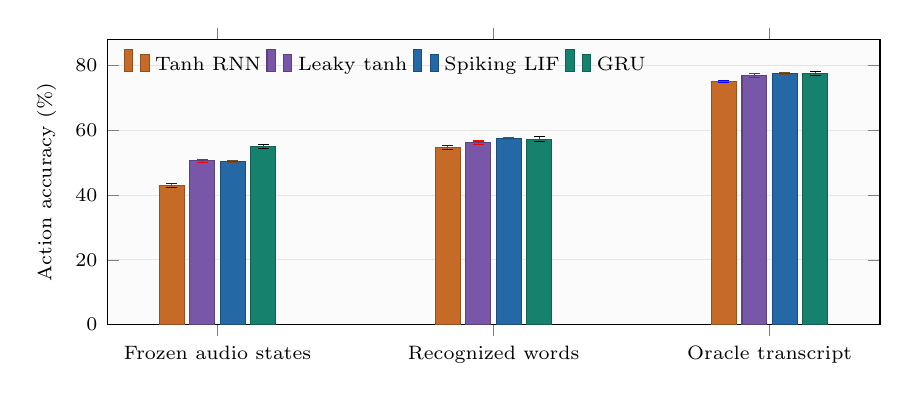
\begin{tikzpicture}
\begin{axis}[ybar,bar width=9pt,width=0.94\textwidth,height=5.2cm,
  ymin=0,ymax=88,ytick={0,20,40,60,80},ylabel={Action accuracy (\%)},
  symbolic x coords={Audio,ASR,Oracle},xtick=data,
  xticklabels={Frozen audio states,Recognized words,Oracle transcript},
  enlarge x limits=0.2,axis background/.style={fill=gray!3},
  ymajorgrids,grid style={gray!20},
  tick label style={font=\scriptsize},label style={font=\scriptsize},
  legend style={font=\scriptsize,draw=none,fill=none,at={(0.01,0.99)},anchor=north west,legend columns=4}]
\addplot+[fill=modelorange,draw=modelorange!75!black,error bars/.cd,y dir=both,y explicit]
  coordinates {(Audio,42.95) +- (0,0.67) (ASR,54.66) +- (0,0.69) (Oracle,75.06) +- (0,0.28)};
\addplot+[fill=modelpurple,draw=modelpurple!75!black,error bars/.cd,y dir=both,y explicit]
  coordinates {(Audio,50.64) +- (0,0.48) (ASR,56.19) +- (0,0.53) (Oracle,77.05) +- (0,0.66)};
\addplot+[fill=modelblue,draw=modelblue!75!black,error bars/.cd,y dir=both,y explicit]
  coordinates {(Audio,50.48) +- (0,0.33) (ASR,57.46) +- (0,0.40) (Oracle,77.53) +- (0,0.37)};
\addplot+[fill=modelgreen,draw=modelgreen!75!black,error bars/.cd,y dir=both,y explicit]
  coordinates {(Audio,55.12) +- (0,0.63) (ASR,57.30) +- (0,0.84) (Oracle,77.59) +- (0,0.52)};
\legend{Tanh RNN,Leaky tanh,Spiking LIF,GRU}
\end{axis}
\end{tikzpicture}%
}}
\caption{SLURP test action accuracy by input representation and recurrent decision core. Bars show five-seed means; whiskers show sample standard deviation. The oracle-transcript condition uses correct corpus text as a diagnostic, not a deployable ASR result.}
\label{fig:accuracy}
\end{figure*}

\begin{figure*}[!t]
\centering
\IfFileExists{risk_coverage.pdf}{%
\includegraphics[width=0.98\textwidth]{risk_coverage.pdf}%
}{\IfFileExists{paper1_action/risk_coverage.pdf}{%
\includegraphics[width=0.98\textwidth]{paper1_action/risk_coverage.pdf}%
}{%
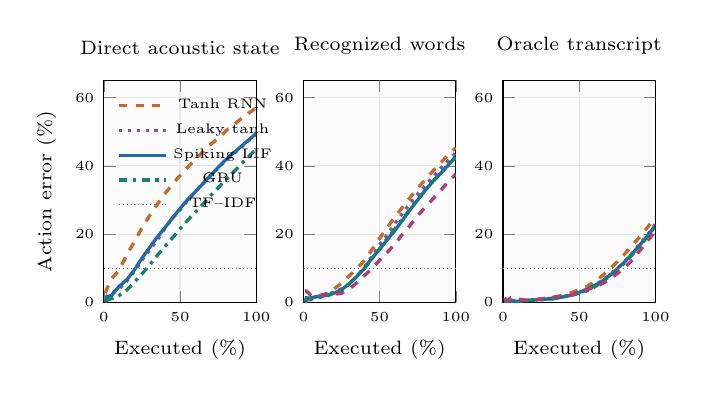
\begin{tikzpicture}
\begin{groupplot}[group style={group size=3 by 1,horizontal sep=0.6cm},
  width=0.29\textwidth,height=4.4cm,xmin=0,xmax=100,ymin=0,ymax=65,
  xtick={0,50,100},ytick={0,20,40,60},xlabel={Executed (\%)},
  grid=major,grid style={gray!18},axis background/.style={fill=gray!3},
  tick label style={font=\tiny},label style={font=\scriptsize},
  title style={font=\scriptsize}]
\nextgroupplot[title={Direct acoustic state},ylabel={Action error (\%)},legend style={font=\tiny,draw=none,fill=none,at={(0.03,0.97)},anchor=north west}]
\addplot[modelorange,very thick,dashed] coordinates {(1,2.69) (2,4.04) (5,6.95) (10,9.44) (15,13.95) (20,17.71) (25,21.82) (30,25.44) (35,28.70) (40,31.81) (45,34.59) (50,37.16) (55,39.58) (60,41.94) (65,44.10) (70,46.24) (75,48.03) (80,50.22) (85,51.96) (90,53.76) (95,55.39) (100,57.05)};
\addplot[modelpurple,very thick,dotted] coordinates {(1,2.02) (2,1.68) (5,2.56) (10,3.97) (15,6.20) (20,9.14) (25,12.40) (30,15.38) (35,18.23) (40,21.65) (45,24.61) (50,27.16) (55,29.83) (60,32.44) (65,34.74) (70,37.10) (75,39.45) (80,41.61) (85,43.46) (90,45.43) (95,47.34) (100,49.36)};
\addplot[modelblue,very thick,solid] coordinates {(1,0.00) (2,1.68) (5,2.02) (10,4.71) (15,6.64) (20,9.50) (25,12.97) (30,16.05) (35,19.13) (40,21.85) (45,24.74) (50,27.46) (55,30.11) (60,32.39) (65,34.80) (70,37.13) (75,39.54) (80,41.79) (85,43.73) (90,45.65) (95,47.55) (100,49.52)};
\addplot[modelgreen,very thick,dashdotted] coordinates {(1,0.67) (2,0.67) (5,1.08) (10,2.02) (15,3.63) (20,5.92) (25,8.34) (30,10.95) (35,13.77) (40,16.27) (45,18.88) (50,21.55) (55,24.05) (60,26.42) (65,28.75) (70,31.27) (75,33.54) (80,35.95) (85,38.15) (90,40.44) (95,42.69) (100,44.88)};
\addplot[modelrose,very thick,dashed] coordinates {};
\legend{Tanh RNN,Leaky tanh,Spiking LIF,GRU,TF--IDF}
\addplot[gray,densely dotted] coordinates {(0,10) (100,10)};
\nextgroupplot[title={Recognized words}]
\addplot[modelorange,very thick,dashed] coordinates {(1,0.00) (2,0.67) (5,0.81) (10,1.34) (15,2.51) (20,3.93) (25,5.60) (30,7.72) (35,9.86) (40,12.29) (45,15.49) (50,18.79) (55,21.95) (60,25.05) (65,27.91) (70,30.73) (75,33.48) (80,35.98) (85,38.53) (90,40.87) (95,43.16) (100,45.34)};
\addplot[modelpurple,very thick,dotted] coordinates {(1,1.35) (2,1.01) (5,1.35) (10,1.75) (15,2.15) (20,2.99) (25,3.98) (30,5.36) (35,7.68) (40,10.29) (45,13.51) (50,16.87) (55,19.86) (60,23.08) (65,26.06) (70,29.11) (75,31.71) (80,34.23) (85,36.74) (90,39.24) (95,41.58) (100,43.81)};
\addplot[modelblue,very thick,solid] coordinates {(1,0.00) (2,1.17) (5,1.35) (10,1.82) (15,2.11) (20,2.68) (25,3.77) (30,5.41) (35,7.57) (40,9.99) (45,12.96) (50,15.56) (55,18.37) (60,21.06) (65,24.07) (70,27.13) (75,30.02) (80,32.87) (85,35.45) (90,37.79) (95,40.20) (100,42.54)};
\addplot[modelgreen,very thick,dashdotted] coordinates {(1,1.35) (2,1.35) (5,0.94) (10,1.48) (15,1.79) (20,2.76) (25,3.62) (30,5.47) (35,7.72) (40,9.95) (45,12.86) (50,15.72) (55,18.74) (60,21.56) (65,24.42) (70,27.30) (75,30.21) (80,32.88) (85,35.47) (90,37.89) (95,40.36) (100,42.70)};
\addplot[modelrose,very thick,dashed] coordinates {(1,3.36) (2,3.36) (5,2.02) (10,2.02) (15,2.47) (20,2.35) (25,2.69) (30,3.92) (35,5.76) (40,7.90) (45,9.86) (50,12.37) (55,14.67) (60,17.04) (65,19.97) (70,22.57) (75,25.49) (80,27.83) (85,30.34) (90,32.79) (95,35.32) (100,37.59)};
\addplot[gray,densely dotted] coordinates {(0,10) (100,10)};
\nextgroupplot[title={Oracle transcript}]
\addplot[modelorange,very thick,dashed] coordinates {(1,0.00) (2,0.00) (5,0.67) (10,0.67) (15,0.63) (20,0.84) (25,1.05) (30,1.34) (35,1.61) (40,2.24) (45,2.87) (50,3.75) (55,4.68) (60,6.04) (65,7.77) (70,9.69) (75,11.92) (80,14.28) (85,16.72) (90,19.35) (95,22.08) (100,24.94)};
\addplot[modelpurple,very thick,dotted] coordinates {(1,1.35) (2,0.67) (5,0.54) (10,0.61) (15,0.54) (20,0.77) (25,0.89) (30,1.14) (35,1.36) (40,1.75) (45,2.15) (50,2.77) (55,3.59) (60,4.96) (65,6.42) (70,8.08) (75,9.97) (80,12.02) (85,14.51) (90,17.23) (95,19.90) (100,22.95)};
\addplot[modelblue,very thick,solid] coordinates {(1,0.00) (2,0.34) (5,0.27) (10,0.34) (15,0.49) (20,0.74) (25,0.86) (30,1.01) (35,1.23) (40,1.66) (45,2.15) (50,2.95) (55,3.81) (60,4.92) (65,6.21) (70,7.89) (75,9.79) (80,11.97) (85,14.35) (90,16.91) (95,19.56) (100,22.47)};
\addplot[modelgreen,very thick,dashdotted] coordinates {(1,0.00) (2,0.00) (5,0.40) (10,0.40) (15,0.54) (20,0.54) (25,0.78) (30,0.90) (35,1.17) (40,1.69) (45,2.07) (50,2.73) (55,3.36) (60,4.53) (65,6.01) (70,7.65) (75,9.64) (80,11.69) (85,14.08) (90,16.63) (95,19.42) (100,22.41)};
\addplot[modelrose,very thick,dashed] coordinates {(1,0.00) (2,0.00) (5,1.35) (10,1.01) (15,0.67) (20,0.50) (25,1.08) (30,1.14) (35,1.72) (40,1.77) (45,2.17) (50,3.16) (55,3.79) (60,4.26) (65,5.48) (70,6.68) (75,8.47) (80,10.26) (85,12.46) (90,15.32) (95,18.12) (100,20.91)};
\addplot[gray,densely dotted] coordinates {(0,10) (100,10)};
\end{groupplot}
\end{tikzpicture}%
}}
\caption{Test action error versus the fraction of decisions executed, ranked by development-calibrated confidence. Recurrent curves show five-seed means; TF--IDF in the text panels is one fit. The dotted line marks 10\% error for orientation; the empirical development threshold used in Table~\ref{tab:slurp} does not guarantee that test risk remains below it.}
\label{fig:risk}
\end{figure*}

\begin{figure}[t]
\centering
\IfFileExists{reliability_asr_snn.pdf}{%
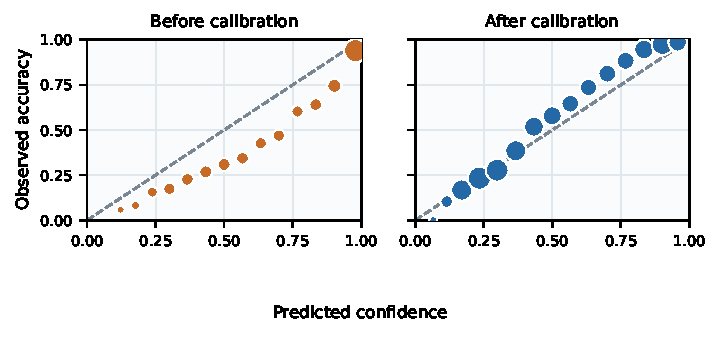
\includegraphics[width=0.98\columnwidth]{reliability_asr_snn.pdf}%
}{%
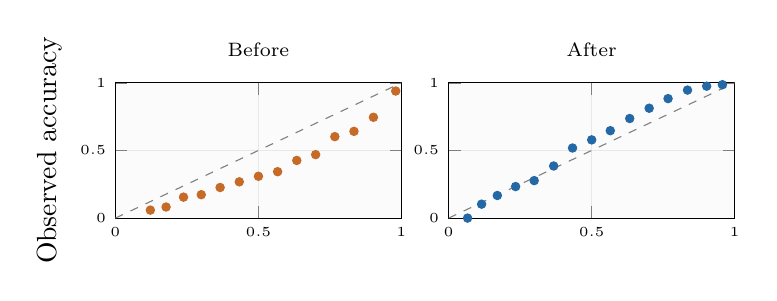
\begin{tikzpicture}
\begin{groupplot}[group style={group size=2 by 1,horizontal sep=0.6cm},
 width=0.43\columnwidth,height=3.3cm,xmin=0,xmax=1,ymin=0,ymax=1,
 xtick={0,0.5,1},ytick={0,0.5,1},grid=major,
 grid style={gray!18},axis background/.style={fill=gray!3},
 tick label style={font=\tiny},title style={font=\scriptsize}]
\nextgroupplot[title={Before},ylabel={Observed accuracy}]
\addplot[gray,dashed] coordinates {(0,0) (1,1)};
\addplot[only marks,mark=*,mark size=1.5pt,modelorange]
 coordinates {(0.122,0.059) (0.177,0.082) (0.238,0.155) (0.300,0.173)
 (0.366,0.226) (0.433,0.268) (0.500,0.309) (0.567,0.343)
 (0.634,0.426) (0.700,0.469) (0.767,0.602) (0.834,0.641)
 (0.902,0.745) (0.980,0.939)};
\nextgroupplot[title={After}]
\addplot[gray,dashed] coordinates {(0,0) (1,1)};
\addplot[only marks,mark=*,mark size=1.5pt,modelblue]
 coordinates {(0.066,0.000) (0.115,0.103) (0.170,0.167) (0.234,0.233)
 (0.299,0.277) (0.367,0.385) (0.433,0.518) (0.500,0.578)
 (0.565,0.646) (0.633,0.736) (0.701,0.812) (0.767,0.883)
 (0.835,0.946) (0.902,0.975) (0.957,0.986)};
\end{groupplot}
\end{tikzpicture}%
}
\caption{Reliability of reference-trained spiking decisions evaluated on ASR words, before and after development-fitted temperature scaling. Each marker is one confidence bin, with predictions from five fixed seeds pooled for display. The diagonal denotes perfect calibration.}
\label{fig:reliability}
\end{figure}

\begin{table}[t]
\caption{Reference-trained ASR-word SLURP calibration and selective risk on test. ECE uses 15 equal-width bins; lower is better. Temperatures are fitted on development data. AURC averages accepted-decision error over coverage ranks. Recurrent rows are five-seed means; TF--IDF is one deterministic fit.}
\label{tab:calibration}
\centering\scriptsize
\begin{tabular}{lrrr}
\toprule
Decision core & ECE before & ECE after & AURC\\
\midrule
Tanh RNN & 0.149 & 0.061 & 0.200\\
Leaky tanh RNN & 0.163 & 0.050 & 0.185\\
Spiking LIF RNN & 0.132 & 0.063 & 0.176\\
GRU & 0.130 & 0.046 & 0.176\\
TF--IDF logistic & 0.203 & 0.028 & 0.149\\
\bottomrule
\end{tabular}
\end{table}

\begin{table}[t]
\caption{French Speech-MASSIVE action accuracy (\%) on 2,031 validated official-validation recordings. The official test split was unavailable. Recurrent values are five-seed means $\pm$ sample standard deviations; TF--IDF is one fit.}
\label{tab:french}
\centering\scriptsize
\begin{tabular}{lrr}
\toprule
Decision core & Acoustic states & ASR words\\
\midrule
Tanh RNN & $42.15\pm0.94$ & $40.29\pm0.45$\\
Leaky tanh RNN & $49.49\pm1.20$ & $41.31\pm1.35$\\
Spiking LIF RNN & $47.56\pm0.98$ & $42.68\pm0.88$\\
GRU & $54.29\pm0.89$ & $44.37\pm0.18$\\
TF--IDF logistic & --- & 50.81\\
\bottomrule
\end{tabular}
\end{table}

\section{Results}
\subsection{Core Accuracy and Replication}
Table~\ref{tab:slurp} and Fig.~\ref{fig:accuracy} report five-seed SLURP test results. With frozen acoustic states, spiking accuracy is $50.48\pm0.33$\%, essentially the same as leak-matched tanh at $50.64\pm0.48$\%. Their paired seed-and-utterance bootstrap 95\% interval for spiking minus leaky tanh is $-1.22$ to 0.98 percentage points. The GRU reaches $55.12\pm0.63$\% (spiking-minus-GRU interval: $-5.93$ to $-3.36$ points), and the one-fit linear probe reaches 51.68\%. Plain tanh reaches 42.95\%, showing why an unmatched leak and initial gain would exaggerate a spiking effect.

The prospectively fixed French acoustic replication in Table~\ref{tab:french} gives spiking 47.56\%, leaky tanh 49.49\%, and GRU 54.29\%. The spiking-minus-leaky-tanh hierarchical interval is $-3.44$ to $-0.36$ points. On French ASR words, spiking averages 42.68\% versus 41.31\% for leaky tanh. Its $+1.37$-point mean lead has a paired seed-and-utterance hierarchical 95\% interval of $-0.01$ to $+2.77$ points, so the directional replication is not decisive. GRU reaches 44.37\% and TF--IDF 50.81\%; the prompt-referenced ASR word error rate is 44.73\%. The French recordings and language differ from SLURP, but the translated 60-intent ontology is related. These accuracies are below the Speech-MASSIVE authors' fine-tuned large-model French results on a different official test split~\cite{speechmassive}; they are decision-core comparisons, not state-of-the-art SLU scores.

On actual SLURP ASR words, spiking, leaky tanh, and GRU reach 57.46\%, 56.19\%, and 57.30\%. The spiking-minus-leaky-tanh hierarchical interval is 0.26 to 2.33 points, a small exploratory lead on this inspected test set; spiking and GRU are close. On oracle transcripts the same cores reach 77.53\%, 77.05\%, and 77.59\%. A word/bigram TF--IDF logistic classifier reaches 62.41\% on ASR words and 79.09\% on oracle text, exceeding every recurrent text core. Recurrence is therefore not necessary for the strongest text score in this protocol. The spiking model loses 20.07 points from oracle to ASR input, with 32.16\% test word error rate. SLURP's original study reported 84.84\% combined scenario--action accuracy on gold text and 78.33\% with its best ASR pipeline~\cite{slurp}; upstream and classifier protocols differ.

Training the text cores on ASR hypotheses from the 11,514 training recordings instead of reference words raises five-seed test accuracy to $56.04\pm0.46$\% for plain tanh, $58.02\pm0.69$\% for leaky tanh, $59.05\pm0.28$\% for spiking, and $58.97\pm0.80$\% for GRU. Training-audio hypotheses have 31.74\% word error rate. The spiking-minus-leaky-tanh hierarchical 95\% interval is $-0.02$ to 2.02 points; the small mean lead is inconclusive over five seeds. Even the best recurrent result remains below the 62.41\% word/bigram classifier on the same test ASR words. This sensitivity check also uses the previously inspected SLURP test set.

\subsection{Confidence, Deferral, and Secondary Task}
Temperature scaling lowers five-seed mean ASR-word spiking ECE from 0.132 to 0.063; Table~\ref{tab:calibration} and Fig.~\ref{fig:reliability} show the calibration change. TF--IDF needs calibration too: its ECE falls from 0.203 to 0.028. Scaling is not uniformly beneficial: French acoustic spiking ECE rises from 0.032 to 0.043. In Fig.~\ref{fig:risk}, the GRU has lower acoustic selective error over most coverage levels. AURC is 0.261 for acoustic spiking versus 0.213 for the GRU, and 0.286 versus 0.215 in French. On ASR words, the recurrent spiking and GRU AURCs are both about 0.176, while TF--IDF is lower at 0.149. The development-selected 10\% error threshold yields only 23.30\% acoustic spiking test coverage and 11.42\% error among accepted actions; it is no test guarantee.

For an illustrative policy, wrong execution costs one, correct execution zero, and deferral $c\in\{0.1,0.2,0.5\}$. We choose each threshold to minimize development cost. At $c=0.2$, always deferring costs 0.2; the best acoustic recurrent core (GRU) costs 0.1723, and the ASR-word spiking core costs 0.1566, executing 32.47\% of requests. TF--IDF is better at 0.1518 cost and 39.91\% execution. These reductions depend on assumed costs, not measured user preferences.

On 100 preloaded SLURP clips, median host-CPU route times are 8.44 ms for acoustic spiking and 111.71 ms for ASR words, with 6.98 points higher accuracy from ASR. Core-only times are 1.17 ms (spiking), 0.62 ms (tanh), and 1.08 ms (GRU); speech observation and energy were not measured.

The EasyCall voice-access stress test remains secondary. Across three speaker-disjoint seeds, spiking accuracy is $46.83\pm1.59$\% versus $45.75\pm2.18$\% for equal-parameter tanh, with a paired speaker-cluster 95\% difference interval of $-1.59$ to 3.76 points. Under a development threshold targeting at most 1\% false execution on noncommands, the spiking core still executes 1.16\% of test noncommands and correctly executes only 7.58\% of commands. Incorrect emergency-call executions occur in every seed. This is a failure boundary, not a deployable accessibility result.

\section{Discussion and Limitations}
Leak matching materially changes the comparison. The spiking core improves on plain tanh but ties leaky tanh on SLURP acoustic states and loses to it on the fresh French recordings. Its recognized-word performance is competitive with a GRU. The mean spiking lead over leaky tanh has the same direction in French, but the hierarchical interval crosses zero; on SLURP, it is sensitive to training input and comes from an inspected test set. A simple nonrecurrent text classifier is stronger in both languages and defers better on SLURP ASR words. The GRU is strongest on both acoustic benchmarks. Thus, these experiments support careful characterization of a spiking decision core, without a general reason to prefer it. Adaptive-threshold spiking units are a concrete next model to test, motivated by speech results in~\cite{yin,bittar}, but no such result is claimed here.

The audio route uses a frozen pretrained speech encoder, and the text route uses full ASR. The acoustic finding applies specifically to a spiking decision head fed 32 pooled, dense vectors from a 39-million-parameter pretrained transformer that has already integrated temporal context; it does not establish how spiking speech processing performs in general. Our earlier hardware-architecture survey~\cite{berhanu_hardware} motivates a separate implementation question; it supplies no energy result for this model. The spiking core's input and readout are analog, its mean hidden firing fraction is about 40\%, and dense CPU operations execute every step. Spike activity is not energy or joules. SLURP has utterance-level labels but no live execution outcomes or changing application context. The French benchmark uses a related ontology and official validation rather than inaccessible official test. EasyCall uses a different front end and fixed intended prompts. No accessibility or clinical efficacy claim follows.

Preliminary SLURP test scores were inspected during pipeline development, including the switch to a frozen encoder; the leak control followed reviewer feedback. The five-seed SLURP intervals therefore remain exploratory. The French acoustic and ASR-text protocols and evaluation split were fixed before their outcomes were inspected, but the corpus shares SLURP-derived semantics. The SNN activity penalty, threshold, and reset also differ from leaky tanh, limiting causal attribution to individual mechanisms.

\section{Conclusion}
A spiking recurrent core can make bounded spoken-action choices and expose a defer option. It does not beat a leak-matched conventional core on either acoustic benchmark, while a GRU is stronger on both. On recognized French words its mean lead over leaky tanh has a seed-and-utterance interval crossing zero. A simple nonrecurrent classifier is stronger on recognized words and gives lower selective risk and simulated action cost on SLURP. The result characterizes a spiking head on dense pretrained speech features; broader spiking speech processing, hardware benefits, and medical efficacy remain untested.

\section*{Code and Data Availability}
Code, result tables, and this manuscript are available at \url{https://github.com/AbielBerhanu/AIxDke2026}. Source datasets remain available from their original providers.

\begin{thebibliography}{16}
\bibitem{slurp} E. Bastianelli, A. Vanzo, P. Swietojanski, and V. Rieser, ``SLURP: A spoken language understanding resource package,'' in \emph{Proc. EMNLP}, 2020, pp. 7252--7262, doi: 10.18653/v1/2020.emnlp-main.588.
\bibitem{speechmassive} B. Lee, I. Calapodescu, M. Gaido, M. Negri, and L. Besacier, ``Speech-MASSIVE: A multilingual speech dataset for SLU and beyond,'' in \emph{Proc. Interspeech}, 2024, doi: 10.21437/Interspeech.2024-957.
\bibitem{representations} E. Villatoro-Tello \emph{et al.}, ``Effectiveness of text, acoustic, and lattice-based representations in spoken language understanding tasks,'' in \emph{Proc. IEEE ICASSP}, 2023, pp. 1--5, doi: 10.1109/ICASSP49357.2023.10095168.
\bibitem{whisper} A. Radford \emph{et al.}, ``Robust speech recognition via large-scale weak supervision,'' in \emph{Proc. ICML}, 2023, pp. 28492--28518.
\bibitem{neftci} E. O. Neftci, H. Mostafa, and F. Zenke, ``Surrogate gradient learning in spiking neural networks: Bringing the power of gradient-based optimization to spiking neural networks,'' \emph{IEEE Signal Process. Mag.}, vol. 36, no. 6, pp. 51--63, 2019, doi: 10.1109/MSP.2019.2931595.
\bibitem{cramer} B. Cramer, Y. Stradmann, J. Schemmel, and F. Zenke, ``The Heidelberg spiking data sets for the systematic evaluation of spiking neural networks,'' \emph{IEEE Trans. Neural Netw. Learn. Syst.}, vol. 33, no. 7, pp. 2744--2757, 2022, doi: 10.1109/TNNLS.2020.3044364.
\bibitem{yin} B. Yin, F. Corradi, and S. M. Boht\'e, ``Accurate and efficient time-domain classification with adaptive spiking recurrent neural networks,'' \emph{Nature Mach. Intell.}, vol. 3, pp. 905--913, 2021, doi: 10.1038/s42256-021-00397-w.
\bibitem{bittar} A. Bittar and P. N. Garner, ``A surrogate gradient spiking baseline for speech command recognition,'' \emph{Front. Neurosci.}, vol. 16, Art. no. 865897, 2022, doi: 10.3389/fnins.2022.865897.
\bibitem{blouw} P. Blouw, X. Choo, E. Hunsberger, and C. Eliasmith, ``Benchmarking keyword spotting efficiency on neuromorphic hardware,'' in \emph{Proc. 7th Annual Neuro-inspired Computational Elements Workshop}, 2019, pp. 1--8, doi: 10.1145/3320288.3320304.
\bibitem{basal} T. Ao, Q. Liu, L. Fu, and Y. Zhou, ``A spiking neural network action decision method inspired by basal ganglia,'' \emph{Procedia Computer Science}, vol. 250, pp. 115--121, 2024, doi: 10.1016/j.procs.2024.11.017.
\bibitem{banad_cloud} R. Ahmadvand, S. S. Sharif, and Y. M. Banad, ``A cloud-edge framework for energy-efficient event-driven control: An integration of online supervised learning, spiking neural networks and local plasticity rules,'' \emph{Neuromorphic Computing and Engineering}, vol. 4, no. 4, Art. no. 044004, 2024, doi: 10.1088/2634-4386/ad8c79.
\bibitem{banad_control} R. Ahmadvand, S. S. Sharif, and Y. M. Banad, ``Neuromorphic robust framework for integrated estimation and control in dynamical systems using spiking neural networks,'' \emph{Scientific Reports}, vol. 15, Art. no. 44753, 2025, doi: 10.1038/s41598-025-28344-4.
\bibitem{guo} C. Guo, G. Pleiss, Y. Sun, and K. Q. Weinberger, ``On calibration of modern neural networks,'' in \emph{Proc. ICML}, 2017, pp. 1321--1330.
\bibitem{selective} Y. Geifman and R. El-Yaniv, ``Selective classification for deep neural networks,'' in \emph{Advances in Neural Information Processing Systems}, vol. 30, 2017.
\bibitem{easycall} R. Turrisi \emph{et al.}, ``EasyCall corpus: A dysarthric speech dataset,'' in \emph{Proc. Interspeech}, 2021, pp. 41--45, doi: 10.21437/Interspeech.2021-549.
\bibitem{berhanu_hardware} A. M. Berhanu, S. Di Jorio, D. T. Worku, S. Sharif, and Y. M. Banad, ``Comparative analysis of neuromorphic hardware architectures for real-time, energy-efficient edge intelligence,'' in \emph{Proc. 2026 Int. Conf. AI x Data and Knowledge Engineering (AIxDKE)}, 2026, pp. 157--161, doi: 10.1109/AIxDKE67294.2026.00035.
\end{thebibliography}
\end{document}
